% begin module natural-exponential-ex7
\begin{frame}
\begin{example} %[Example 6, p. 277]
\begin{columns}[c]
\column{.4\textwidth}

\psset{xunit=0.5cm, yunit=0.5cm}
\begin{pspicture}(-5,-1)(5.5,10)
\psframe*[linecolor=white](-5,-1)(5.5,10)
\tiny
\psaxes[ticks=none, labels=none]{<->}(0,0)(-5,-1)(5,9.4)
\fcLabels{5}{9.4}
\fcXTickWithLabel{1}{$1$}
\fcXTickWithLabel{-1}{$-1$}
%Function formula: (e)^{(1)/(x)}
\uncover<6-20>{
\psplot[arrows=->, linecolor=\fcColorGraph, plotpoints=1000] {0.45} {0.55} {2.718281828 1 x div exp }
}
\uncover<20->{
\fcFullDot{-0.5}{0.135335283}
}
\uncover<10-20>{
\psplot[arrows=->, linecolor=\fcColorGraph, plotpoints=1000] {3.5} {5} {2.718281828 1 x div exp }
}
\uncover<21->{
\psplot[linecolor=\fcColorGraph, plotpoints=1000] {-5} {-0.01} {2.718281828 1 x div exp }
\psplot[linecolor=\fcColorGraph, plotpoints=1000] {0.45} {5} {2.718281828 1 x div exp }
\rput(2.3,3){$y=e^{\frac1x}$}
}
\uncover<10-20>{\psplot[arrows=->, linecolor=\fcColorGraph, plotpoints=1000] {-4.95} {-4} {2.718281828 1 x div exp }
}
\uncover<8-20>{
\psplot[linecolor=\fcColorGraph, plotpoints=1000] {-1.4} {-0.7} {2.718281828 1 x div exp }
\psplot[arrows=>-, linecolor=\fcColorGraph, plotpoints=1000] {-0.7} {-0.01} {2.718281828 1 x div exp }
}
\uncover<10->{
\psline[linecolor=\fcColorTangent, linestyle=dashed] (-4.95,1) (5,1)
\rput[t](4,0.9){$y=1$}
}
\end{pspicture}

%\ \only<handout:0| -5>{%
%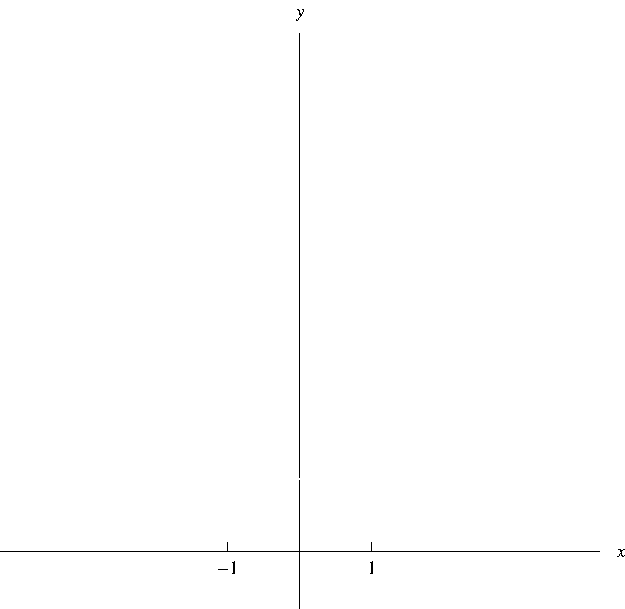
\includegraphics[height=5cm]{exponential-functions/pictures/07-02-ex7a.pdf}%
%}%
%\only<handout:0| 6-7>{%
%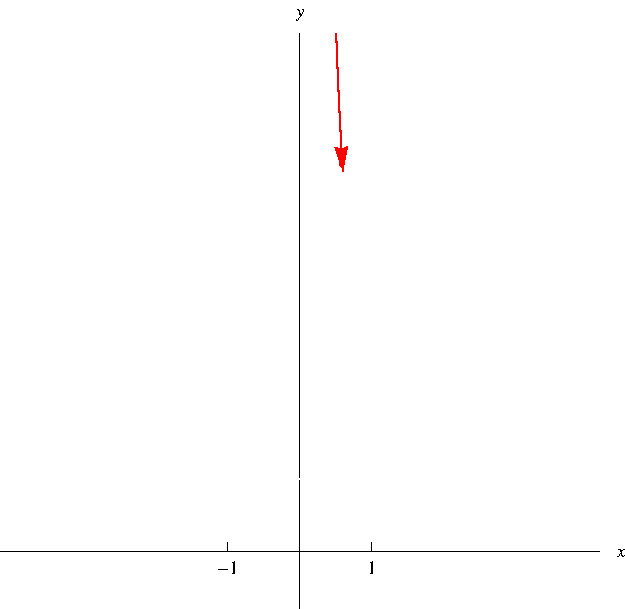
\includegraphics[height=5cm]{exponential-functions/pictures/07-02-ex7b.pdf}%
%}%
%\only<handout:0| 8-9>{%
%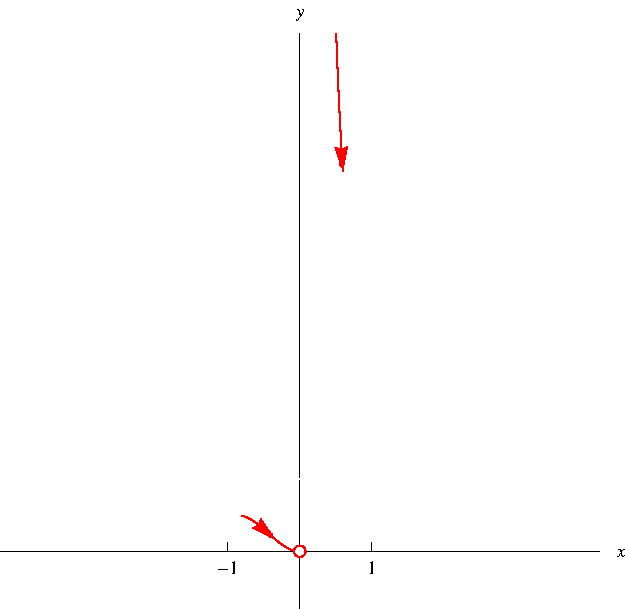
\includegraphics[height=5cm]{exponential-functions/pictures/07-02-ex7c.pdf}%
%}%
%\only<handout:0| 10-20>{%
%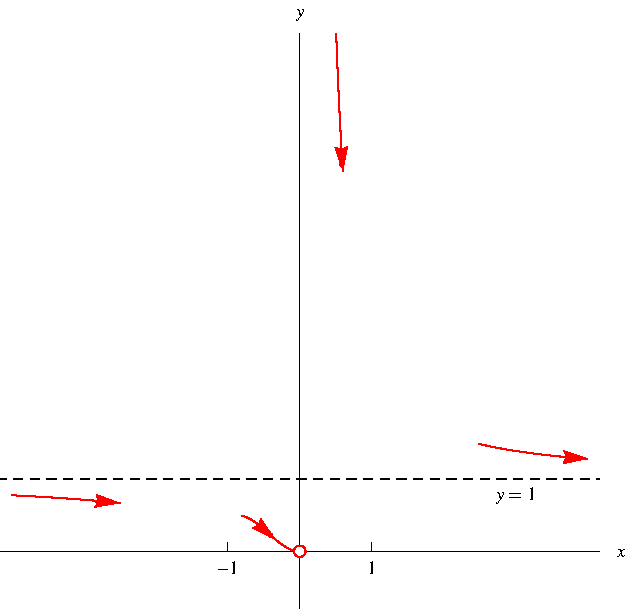
\includegraphics[height=5cm]{exponential-functions/pictures/07-02-ex7e.pdf}%
%}%
%\only<21->{%
%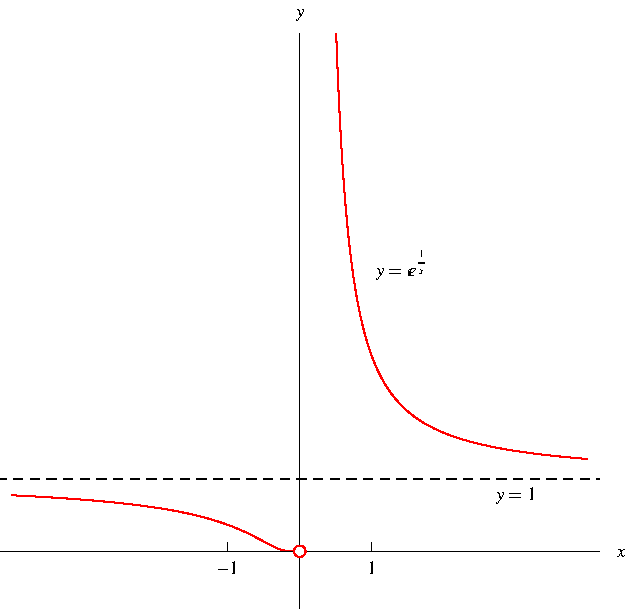
\includegraphics[height=5cm]{exponential-functions/pictures/07-02-ex7f.pdf}%
%}%
\column{.6\textwidth}
\qquad Draw the graph of $f(x) = e^{1/x}$.
\begin{itemize}
\item<2->  $f(x)$ is always positive.
\item<3->  Domain: everything but 0.
\item<4->  Check for vertical asymptote at 0.
\item<4->  $\displaystyle t = 1/x: \lim_{x\rightarrow 0^+} e^{1/x} \uncover<5->{ = \lim_{t\rightarrow\infty}e^t} \uncover<6->{ = \infty .}$
\item<4->  $\displaystyle t = 1/x: \lim_{x\rightarrow 0^-} e^{1/x} \uncover<7->{ = \lim_{t\rightarrow -\infty}e^t} \uncover<8->{ = 0.}$
\item<9->  As $x\rightarrow \pm \infty$, $1/x \rightarrow 0$.
\item<10->  Therefore $\lim_{x\rightarrow \pm \infty} e^{1/x} = 1$
\item<10->  $y = 1$ is a horizontal asymptote.
\end{itemize}
\end{columns}
\abovedisplayskip=0pt
\belowdisplayskip=0pt
\abovedisplayshortskip=0pt
\belowdisplayshortskip=0pt
\begin{align*}
\uncover<11->{f'(x) } & \uncover<11->{ = e^{1/x}\alertNoH{ 12-13}{(1/x)'}} \uncover<12->{ = e^{1/x}\alertNoH{ 12-13}{( \uncover<13->{-x^{-2}} )}} \uncover<14->{ = \alertNoH{ 17-18}{-e^{1/x}/x^2}.} \\
\uncover<15->{f''(x)} & \uncover<15->{ = -\frac{(x^2) ( - e^{1/x}/x^2) - (e^{1/x})(2x)}{x^4}} \uncover<16->{ = \alertNoH{ 19-20}{\frac{e^{1/x}(1+2x)}{x^4}}.}
\end{align*}
\alertNoH{ 18}{\uncover<18->{Always decreasing.}}  \alertNoH{ 20}{\uncover<20,21->{Inflection point: $(-1/2, e^{-2})$.}}
\end{example}
\end{frame}
% end module natural-exponential-ex7
